\chapter{SleeveAR}
\label{sec:sleevear}

\section*{Summary}

This chapter describes a new approach to deal with the various SleeveAR implementation challenges, and  identifies the critical resources required for a successful implementation.

\todo{Artur: "establish the most important requirements and objectives to be achieved by the solution" - isto deve ser feito logo na intro, em Requirements and Goals, e não aqui.}


\section{Vision}
\label{sec:sleevear:approach}

SleeveAR has ambitious goals, aiming further beyond the accomplishments achieved by LightGuide. 
As described in the previous section, LightGuide only focused on projecting information on top of the hand. Not only does this leaves a small room for movement diversity, but also reduces the amount of possible and useful information that can be given.
By increasing the projection area throughout the whole arm and user's surrounding environment areas, we can successfully improve an user's awareness while a movement is being executed. 
\todo{em vez de 'not only that, blah blah blah, ser por ex. "IN ADDITION, if it was possible for the movement THAT IS being replicated to be...} Not only that, but if it was possible for the movement being replicated to be originated by another person, we could achieve a much more realistic and useful guidance.
With SleeveAR, virtual content can be projected onto different surfaces, and even, onto people's own limbs, to provide, in real-time, a more immersive experience. 

Our vision consists of two main concepts. Firstly, the precise recording of the exercise being demonstrated by a personal therapist. 
And secondly, the ability to properly guide another person, the rehabilitation subject, during the execution of the pre-recorded exercise.
Hereafter we will describe in detail each of this general concepts of our vision.

%While, at the same time, provide awareness of the rehabilitation exercise progress to insure the correctness of the patient's movements.
%With SleeveAR, a therapist can easily demonstrate the prescribed exercises and make sure his patient will perform them correctly without the requirement of his close supervision.

%In the SleeveAR system, the exercise being performed needs to be recorded beforehand, which, in this case, should be a health professional. 
%Not only it provides a great range of possible movements, but also assigns,onto the professional, the responsibility of providing adequate exercises based on a specific patient's condition.




\section{Process (Or SleeveAR Workflow)}


\todo{explicar 3 fases}


\subsection{Recording}

Usually, the patient's prescribed exercises were specifically conceived designed for the current patient's health condition. 
With this in mind, we wanted to maintain this relation between a therapist and a patient, by giving the therapists the power for demonstrating the prescribed exercises to the patient. 
Based on this demonstration, SleeveAr will capture the therapist movement, and it will build and store its model for a later usage.
By giving the therapist the responsibility of demonstrating the exercise, we do not need to worry about the physical limitations of the patient that would use our system to recreate it. 
We are assuming the recorded exercise is already customized for the patient in question.

Given these assumptions, SleeveAr must then be able to guide a patient through those exercises as best as it can. Next we describe the behaviour SleeveAR should have while guiding a patient.


\subsection{Guiding}

Guiding a patient through an exercise can be divided in three phases in our approach, which are as follows:

\begin{itemize}
\item Reaching Initial Position
\item Performing Exercise
\item Performance Review
\end{itemize}

We consider these three phases to be a simple and clear way of organizing what SleeveAR should do when interaction with an patient.
To successfully recreate an exercise, we considered the user must first reach the exercise initial position, i.e., the first arm position from the recorded demonstration.
To do this, a patient must follow SleeveAR's feedback in order to achieve the correct arm position. 
All feedback used for this first phase is explained in section \ref{sec:feedback}.
After SleeveAR considers the initial position has been reached, we can now start guiding the user through the remaining exercise.

It could be an almost impossible task for a patient to recreate an exercise exactly the same as the original. 
With this in mind, SleeveAR needs to rely on thresholds for specific values. 
By doing so, if it was required of a patient to achieve, for example, a 90 degree arm flexion, he would not 
need to actually achieve it, being only enough for him to get close to that degree of flexion.

Finally at the end of each exercise, SleeveAR should provide an overview of the patient's performance in comparison with the original. 
This will help the patient understand what he might have done wrong and in which parts of the exercise he could still perform better.

To successfully guide a patient through his exercises while informing him of his performance, we need to plan how will SleeveAR interact with its users. 
Next section will describe our planned designs for providing real-time and interactive feedback aimed at the user.


\subsection{Performance Review}

\begin{figure}
    \begin{center}
        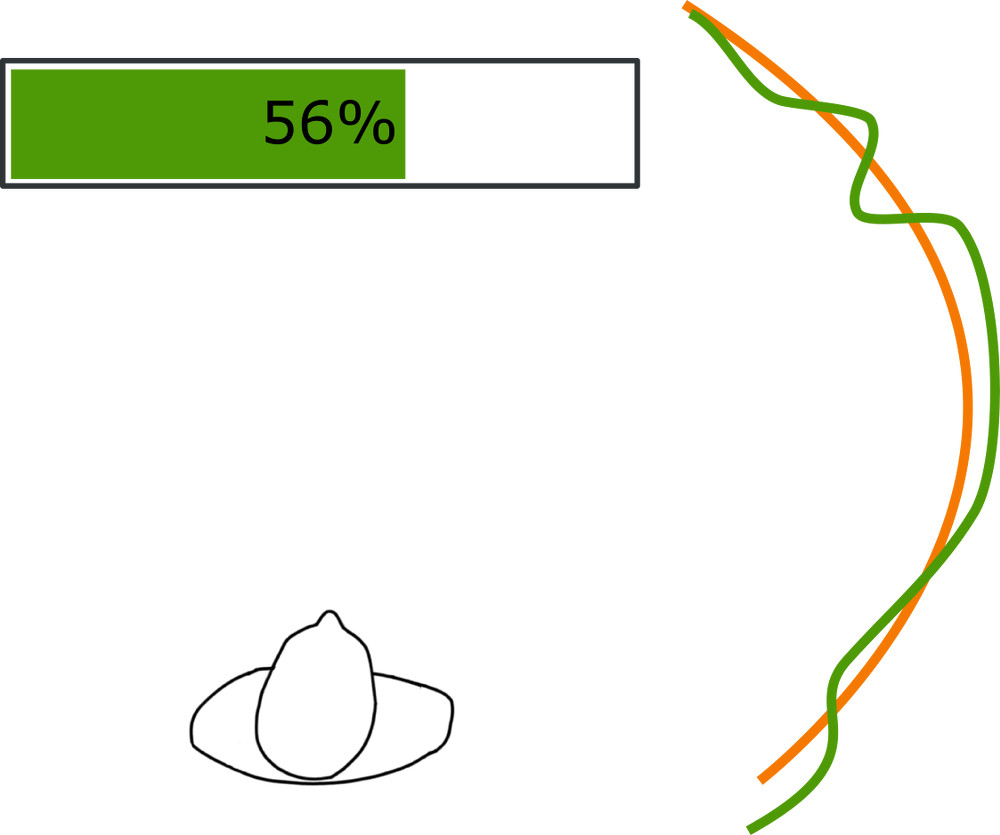
\includegraphics[width=0.35\textwidth]{imgs/approach/performancereview}
    \end{center}
    \caption{Performance Review.}
    \label{fig:performancereview}
\end{figure}

Whenever an exercise is finished, SleeveAR must provide users with a review of their performance. 
By reviewing their exercise, a patient would be able to understand how close he was from the original exercise.

Patients will be informed about their performance by two different designs. 
First, and perhaps most importantly, the original exercise trajectory will be drawn on the floor, followed by the user's recently executed attempt. 
These trajectories will help to visualize what fractions of the exercise could use improvement.
Second, a score will be calculated, based on similarity between both movements, and also projected on the floor. 
With this small gamification, users will feel motivated to improve their score and, consequently, also improve their overall performance.

On figure \ref{fig:performancereview}, we have an example where an orange and green line, 
respectively representing the original trajectory and user's attempt, are drawn on the floor. 
The calculated score would be shown with a simple horizontal bar, including the calculated percentage of similarity.


\section{Feedback}
\label{sec:feedback}


\todo{introduzir}


\subsection{Visual Feedback}
\label{vision-feedback}


\begin{figure}[!t]
\minipage[t]{0.49\textwidth}
  \centering
  \includegraphics[width=0.7\linewidth]{imgs/approach/elbowangle}
    \caption{Elbow Angle Definition.}
    \label{fig:elbowangle}
    \endminipage\hfill
\minipage[t]{0.49\textwidth}
  \centering
  \includegraphics[width=0.9\linewidth]{imgs/approach/forearmfeedback}
    \caption{Fore Arm Visual Feedback.}
    \label{fig:forearmfeedback}
    \endminipage
\end{figure}



%\begin{figure}[!t]
%    \begin{center}
%        \includegraphics[width=0.5\textwidth]{imgs/elbowangle.png}
%    \end{center}
%    \caption{Elbow Angle Definition.}
%    \label{fig:elbowangle}
%\end{figure}

Providing useful and minimalist design was our goal when designing our visual feedback. There were some key points we wanted to address when designing it.
First of all, the visual information had to provide the user with a representation of his \textbf{current} position, while also showing the \textbf{desired} position. 
These representations had to be done in a way the user would easily comprehend what to do in order to achieve that same desired position.
To provide suitable feedback regarding the full arm we first applied different design for each of the regions. Next we will present our planned visual feedback designs.

\subsubsection{Fore Arm}

Before creating the fore arm visual feedback it was important to understand what type of movement could be executed with this arm region.
The fore arm is connected to the upper arm by the elbow joint and its range of motion could be summarized in extension and flexing of the arm.
When extending or flexing the arm, we basically are changing the elbow angle, given by the angle between the upper and fore arm.
If we look at figure \ref{fig:elbowangle} we can see an example of two different elbow angles. 
On the left, we see an elbow angle $\theta$$_1$ of approximately 180 degrees, while on the right an elbow angle $\theta$$_2$ of 90 degrees.  

As we said previously, we wanted both designs to represent the current and desired state. 
Our final design for a fore arm feedback makes use of a circle with two bars, similar to a clock with two pointers.

%\subsubsection{Current State}

%\begin{figure}[!t]
%    \begin{center}
%        \includegraphics[width=0.5\textwidth]{imgs/forearmfeedback.png}
%    \end{center}
%    \caption{Fore Arm Visual Feedback.}
%    \label{fig:forearmfeedback}
%\end{figure}

To represent the current state, we use the black bar, seen in figure \ref{fig:forearmfeedback}. Whenever the user moves his fore arm, this bar will move accordingly.
On the other hand, the desired fore arm state is represented by the green bar. 
For the user to achieve this state, is is required of him to move his fore arm in order for the black bar to reach the green bar.

To extend the user's awareness we added two additional features specifically to this design. 
Depending on the distance between both bars, the circle color would fade between red, too far, and green, close enough. 
Also, if the black bar gets too far from the desired position, rotating arrows will appear to wan the user he is currently not correctly positioned. 
Next we present the planned design for the upper arm feedback.

\subsubsection{Upper Arm}

\begin{figure}[!t]
    \begin{center}
        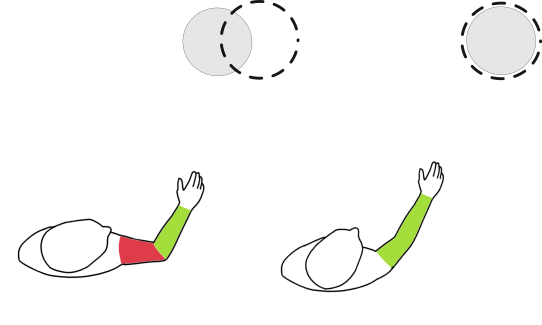
\includegraphics[width=0.5\textwidth]{imgs/approach/upperarmfeedback}
    \end{center}
    \caption{Upper Arm Visual Feedback.}
    \label{fig:upperarmfeedback}
\end{figure}

As for the upper arm region, the type of movement allowed can be represented by the direction it is pointing to, 
which is obtained by a direction vector from the shoulder to the elbow as seen in fig \todo{figura}.
Once again, it was necessary for the design, seen at fig \ref{fig:upperarmfeedback} to both show the current and desired state. 

%\subsubsection{Current State}

To represent the upper arm current direction, a dotted circumference was chosen. 
By moving the upper arm vertically or horizontally, the dotted circumference should move, respectively, vertically and horizontally.

%\subsubsection{Desired State}

As for the desired state, a simple circle was chosen. 
For the upper arm to achieve the desired direction the user simply has to move it until the dotted circumference surrounds the circle.

\subsubsection{Full Arm}

\begin{figure}[!t]
    \begin{center}
        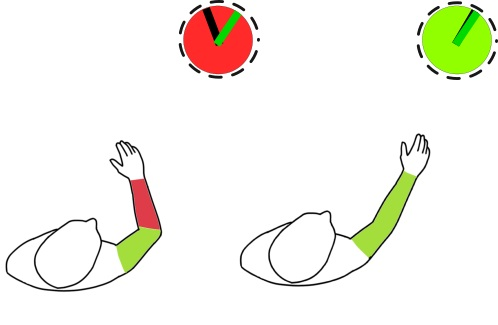
\includegraphics[width=0.4\textwidth]{imgs/approach/fullarmfeedback}
    \end{center}
    \caption{Full Arm Visual Feedback.}
    \label{fig:fullarmfeedback}
\end{figure}

Each one of the previously presented designs are able to guide each arm region individually.
In order to guide a user to a full arm position, we combined both of them as seen on fig \ref{fig:fullarmfeedback}.

By replacing the grey circle, used on the upper arm's design, with the elbow angle circle from the fore arm's design, we are able to use both of them simultaneously. 

All these designs are able to guide the user to a specific, but static, position. For us to be able to guide a user throughout a movement, there need to be some changes on it.

In addition to the already presented feedback, which will be projected on the floor, we will also project information on top of the user's arm. 
In this case, we will not provide feedback as detailed as it is being provided on the floor. 
Instead, we will project diferent colors in each arm region depending on how far they are from the desired state. 
Once again, looking at figures \ref{fig:forearmfeedback}, \ref{fig:upperarmfeedback} and \ref{fig:fullarmfeedback}, we can observe the 
different arm regions having different colours on top, depending on the user's arm position.
These arm color projections will help in highlighting what the user might be doing incorrectly without losing focus on the main feedback.

\subsubsection{Movement Guidance}
\label{sec:movementguidance}
During an arm movement, we can not assume that both the upper and fore arm will remain the same. 
We can have an example were the arm remains fully extended throughout the movement or where the fore arm varies during the movement. 
In this case there's an elbow angle variation which mean the fore arm desired state is continuously changing.
With this in mind, our planned feedback must then change its desired state during the movement.

As for the upper arm, to help the user know to where he must move it, a path will be drawn showing the direction to where he must go. 
If we look closely at the previously presented design, we can observe it actually focus around the circle. 
The fore arm changes the circle itself, while the upper arm controls the dotted circumference that must cover also the circle. 
With this in mind, if we move this same circle through the movement path, we will be able to continuously inform the user about the 
desired direction while also updating what specific elbow angle he should have. 
In fig \ref{fig:movementguidancefeedback} we can see an example where the user is already midpoint in the exercise.



\begin{figure}[!t]
    \begin{center}
        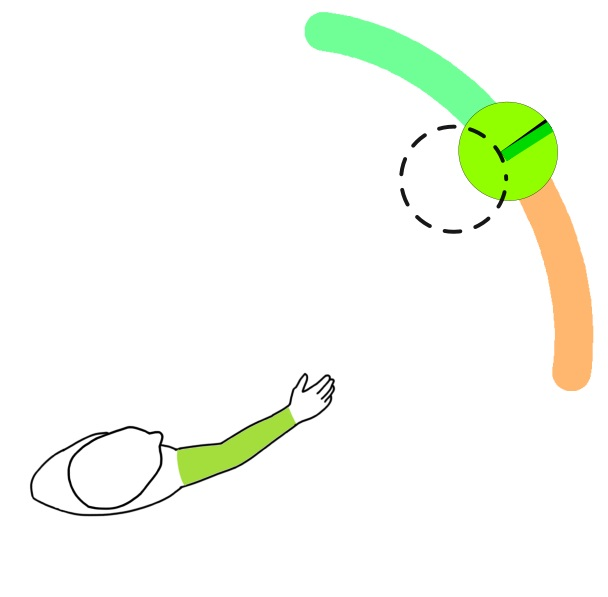
\includegraphics[width=0.4\textwidth]{imgs/approach/movementguidancefeedback}
    \end{center}
    \caption{Movement Visual Feedback.}
    \label{fig:movementguidancefeedback}
\end{figure}

%\begin{figure}[!b]
%    \begin{center}
 %       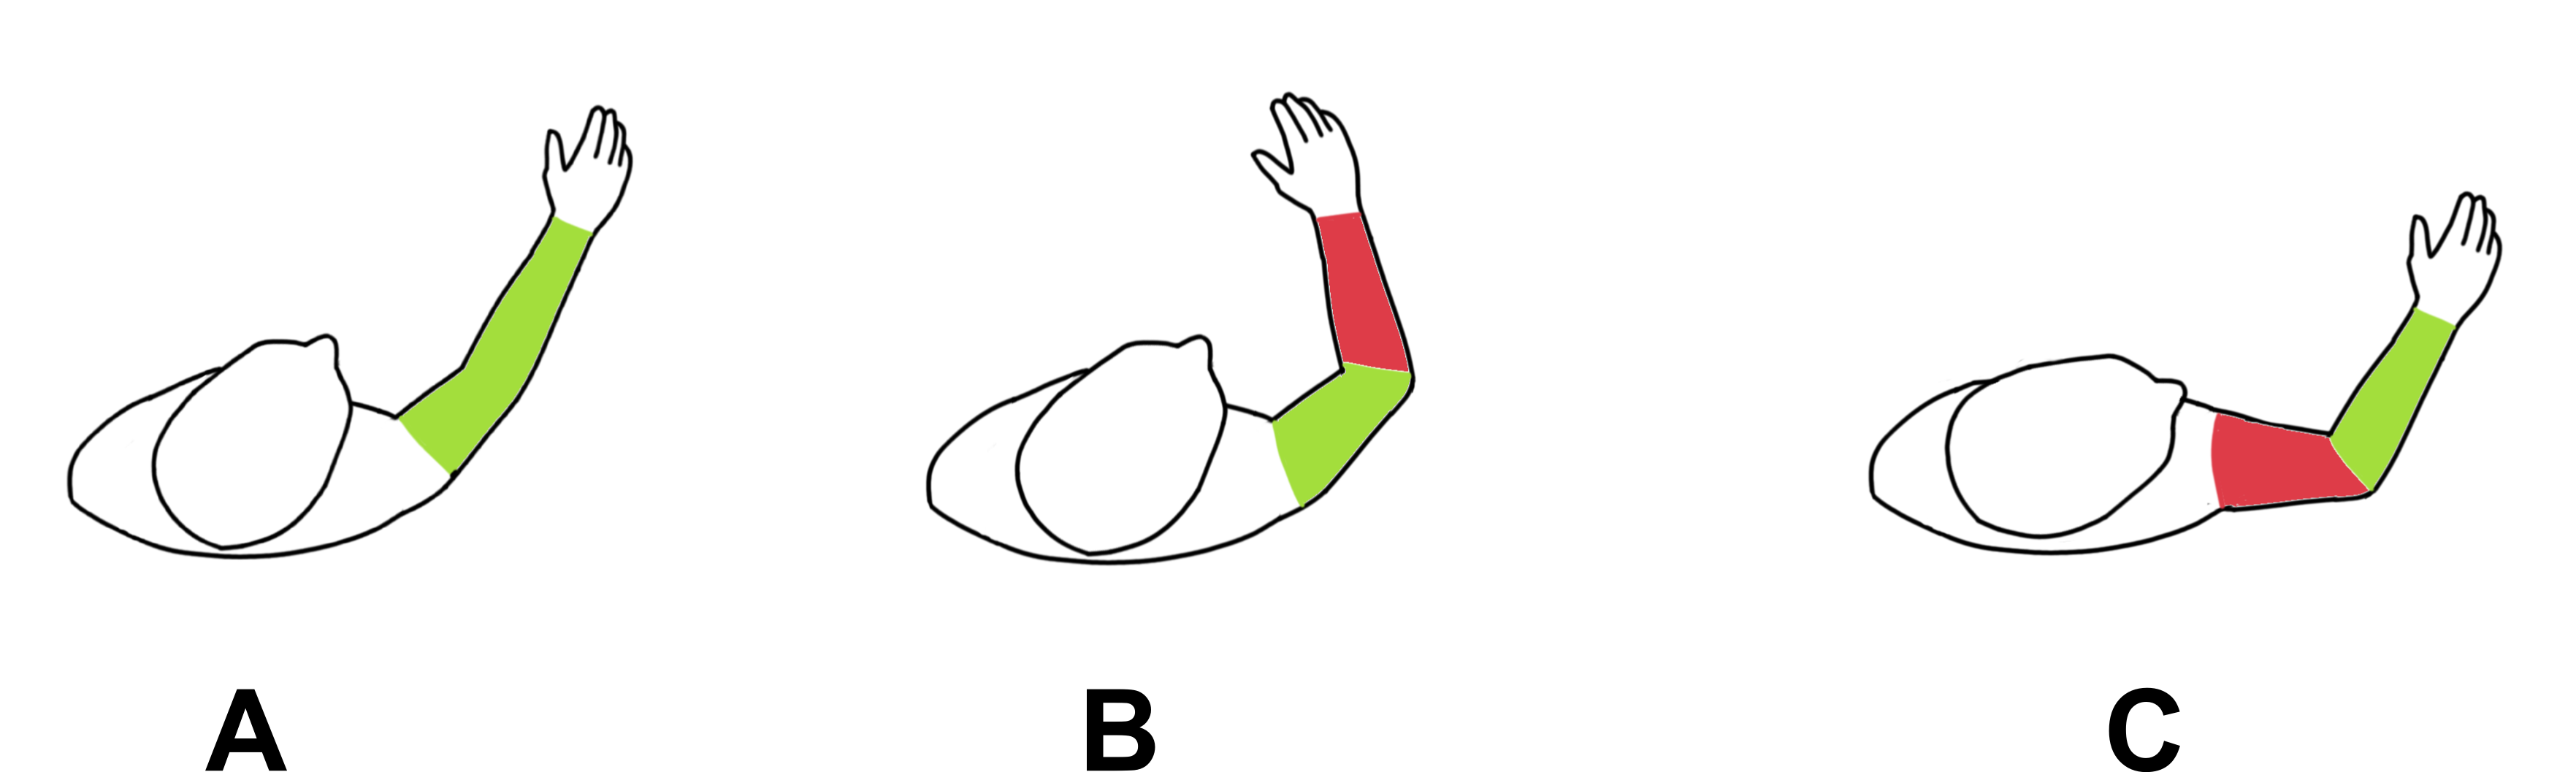
\includegraphics[width=0.4\textwidth]{imgs/armvisualfeedback.png}
  %  \end{center}
   % \caption{Sleeve Projected Feedback: A) Correct Arm. B) Incorrect Fore Arm. C) Incorrect Upper Arm}
%    \label{fig:armvisualfeedback}
%\end{figure}

\subsubsection{Floor Guidance}
\todo{este ja n faz mt sentido}

\subsection{Audio}